\documentclass[a4paper,12pt]{article}
\usepackage[T1]{fontenc}
\usepackage[latin1]{inputenc}
%\usepackage[polutonikogreek]{babel}
%\usepackage{ngerman} %deutschtrennung
\usepackage{amssymb} %math-befehle
\usepackage{fancyhdr} %kopf- und fusszeile
\usepackage{a4wide}
\usepackage[top=20mm]{geometry} %seitenraender
%\usepackage[paper=a4paper,left=25mm,right=25mm,top=20mm,bottom=25mm]{geometry} %seitenraender
\usepackage{parskip} %kein einzug bei absatz
\usepackage[pdftex]{graphicx} %fuer grafiken einfuegen
\usepackage{color}
\definecolor{LK}{rgb}{0.05,0.05,0.3} %dunkelblau
\usepackage[pdftex,bookmarks=true,bookmarksnumbered=true,colorlinks=true,linkcolor=blue,filecolor=red,citecolor=LK,pdfstartview=FitH]{hyperref} %kapiteldarstellung im pdf file
\renewcommand{\textfraction}{0.15} %lockerere bildpositionierungsregeln
\renewcommand{\topfraction}{0.85}
\renewcommand{\bottomfraction}{0.65}
\renewcommand{\floatpagefraction}{0.60}
\renewcommand{\figurename}{Fig.} %statt Abbildung steht nur Abb. bei bildern
\newcommand{\Matrix}[2]{\left(\begin{array}{#1}#2\end{array}\right)}
\setcounter{topnumber}{3}
% \addto\captionsngerman{%
 %   \renewcommand{\figurename}{Fig.}%
   % \renewcommand{\tablename}{Tab.}%
  %}



\begin{document}
%%%%%%%%%%%%%%%%%% title page %%%%%%%%%%%%%%%%%%%%%
\pdfbookmark[1]{title page}{tit}

\title{IBIS data reduction, v170413}

\author{Lucia Kleint \\
e-mail: \mbox{kleintl@ucar.edu}
}

\date{April 13, 2017}

\maketitle
\newpage
%%%%%%%%%%%%%%%%%%%%%%%%%%%%%%%%%%%%%%%%%%%%%%%%%%%%

\tableofcontents
\newpage

%%%%%%%%%%%%%%%%%%%%%%%%%%%%%%%%%%%%%%%%%%

\section{Introduction}
\subsection{General}
The IBIS data reduction can be done (more or less) automatically using ibis\_gui\_new.pro. Start with:

IDL> ibis\_gui\_new

The required libraries (see requirements) must be in your !Path variable. The first button of the GUI needs to be pressed each time the GUI (idl session?) is started to initialize all variables. The variables that must be changed for each reduction are hardwired in this program (which creates ibis\_variables.txt
for an easier access in future reduction steps) and in textbox\_lk.pro.

The other buttons/programs should be run in this order but one may stop
in the middle and continue on the next day as long as the first button
is always used.

The wavelength to reduce is defined when clicking on 'variables'. 
Some parameters (for example kernel size and type of destretch) will
be the same for all wavelengths during one run of the GUI, i.e. if
you define lambda=[8542 6302]. If you want different parameters for
each wavelength, define lambda=[8542] first, run the full reduction,
define lambda=[6302] and re-run the reduction with the different
settings. One also needs to pay attention if for example the exposure
time changed during the day (only one dark will be created, so rerun
the reduction for other dark and corresponding observations).

The kernel size for the destretch is written in kerneltxt.txt. The program checks if
the file exists. If yes, use values in txt file, if not, use [0,64,32,16].

Generally, if there is an overwrite option this means that the first
run of the subprograms will create all necessary files (even for $\lambda$
that were not specified in the beginning). Re-running and setting the
overwrite option should not be necessary in general.

If the polcal was taken on a different date, specify its path in first
textbox (all subdirectories will be searched). Format should be
similar to 'path to original data', which will be chosen in case
polpath is not defined in the textbox.

Starting with v4, a complete .tex log of all data reduction steps and
important images is created in a subdirectory called \textit{log}. You
need to manually do \textit{latex log\_datared.tex} (often more than
once to get the labels right), then \textit{dvips log\_datared.dvi}
and \textit{ps2pdf log\_datared.ps}. Sometimes the \textit{clearpage}
command will need to be inserted if the compilation is not working. This may happen when many images were inserted with little text (for example when one reduces a dozen timestamps).

This version of the GUI no longer supports pre 2010 data (that were
taken with a different camera and a different file system). v5 of the
GUI works fine for those. The main change from v5 to this version (newred) is
the alignment: now all data in all wavelengths should be aligned in
the end. Currently, IBIS creates one fits file per scan and all
images, filters, polarization states are in extensions. Also new is
the possibility to run the polcal with fewer than 4 table positions. I
verified that even just one table position gives the same X matrix
(using 2 positions still recommended).

Many subprograms were taken from A.~Tritschler's version of the data reduction but there are significant differences in programming, user handling and variable names, so that the two versions are not compatible. Major differences between the two versions include a totally rewritten polcal by T. Schad (with the same X matrices as result) and minor differences in beam combination, size of speckle files, the alignment procedure and various bug fixes. Also, the prefilter is now applied to the gain (as of June 2015) and thus all data are corrected for the prefilter automatically.

\subsection{Requirements}

All necessary routines should already be included in the ibis\_newred directory and its subdirectories. All you need to do is to also include the subdirectories in the IDL path and adapt ftsread.pro for the absolute path to fts\_cent.dat.

textbox\_lk.pro (which opens a widget in this widget to manually
         select paths etc.) \\
          coyote library (fanning) \\
          mpfitellipse (directory called 'fitting') -> move to your idl path\\
          buttonbox\_lk.pro\\
          xline, yline, diffelement, xy, anim\_lk (for other routines)\\
          astrolib (for find\_all\_dir etc.) 
                       (downloaded from: http://idlastro.gsfc.nasa.gov/ftp/) \\
          where2d (ssw) 2-dimensional where\\
          several routines from solarsoft (directory called fromssw) \\
          ftsread.pro (adapt the absolute path to fts\_cent.dat in the routine!)

\subsection{ToDo and known problems}

\begin{itemize}
 \item setting 'limb' requires some modifications and will currently stop/crash. The option assumes\\
      a) the limb is vertical in the image\\
      b) there is a sunspot located at some fixed coordinates which must be changed manually 
         (to avoid center-to-limb calculation at that point). change in: \mbox{ibis\_reduce\_speckle.pro:154} and
            ibis\_calibrate.pro:447
     limb does not work with the new camera yet!

\item ibis\_combine\_lk: keywords scan\_no=5, Nmax=30, /ATM, /daydrift, /movie not set!!!
\item spectroscopy and single beam polarimetry not done yet for speckle version of new cam
\item reduce required memory for ibis\_gui.pro -> 4 GB RAM not enough...
\item cog blueshift seems to be better than poly\_fit for new cam (which has fringes). But for 6302 poly\_fit seems better.
\item speckle for new cam makes 1 burst per wl per fits file. There
  should be at least 50 images per filter (=more than ~8 wl steps for polarimetry) for successful speckle. ToDo: Option to combine/split files for speckle
\item ibis\_flat\_avg\_nb could be faster: read s000 only (once per
  timestamp) and assume that other files (per timestamp) are the same
\item assign\_speckle2nb does not have an overwrite option. Must delete file manually if redoing speckle.
\item option R>1, i.e. repetitions of same line in fits file not supported yet
\item autopolcal: BE CAREFUL! the labels of the buttons are suggestions, taking poldir[0,28,56,84]
    which usually will not be okay since the instrument fails at least once per calibration sequence
    and/or the series are restarted by the observers due to clouds etc.. For example, on June 12 the 
    first poldir series was also useless (which was not easily visible in the logs! the hint was that the
    log said "Iteration  \#1 of 10" instead of '\#1 of 1') so really make sure you choose the 
    correct starting directories. Currently, there is no warning if something looks strange.
\item to look at the reduced data, use view\_ibis,stokesout,lambda=wl\_obs (will be implemented in gui later)
\item the parallelization through bridges is not entirely stable. If you ever had to do Ctrl+c before `reduce IBIS' to get to the command line, the bridges will quit and need to be re-run (=do reduce IBIS again). Also, never do Ctrl+C while the bridges are running, otherwise you'll need to kill the whole terminal.
\end{itemize}

\section{The GUI}
\label{sec:gui}
Each subsection deals with one button of the GUI, as shown in Fig.~\ref{figgui}.

\begin{figure}[!htb]
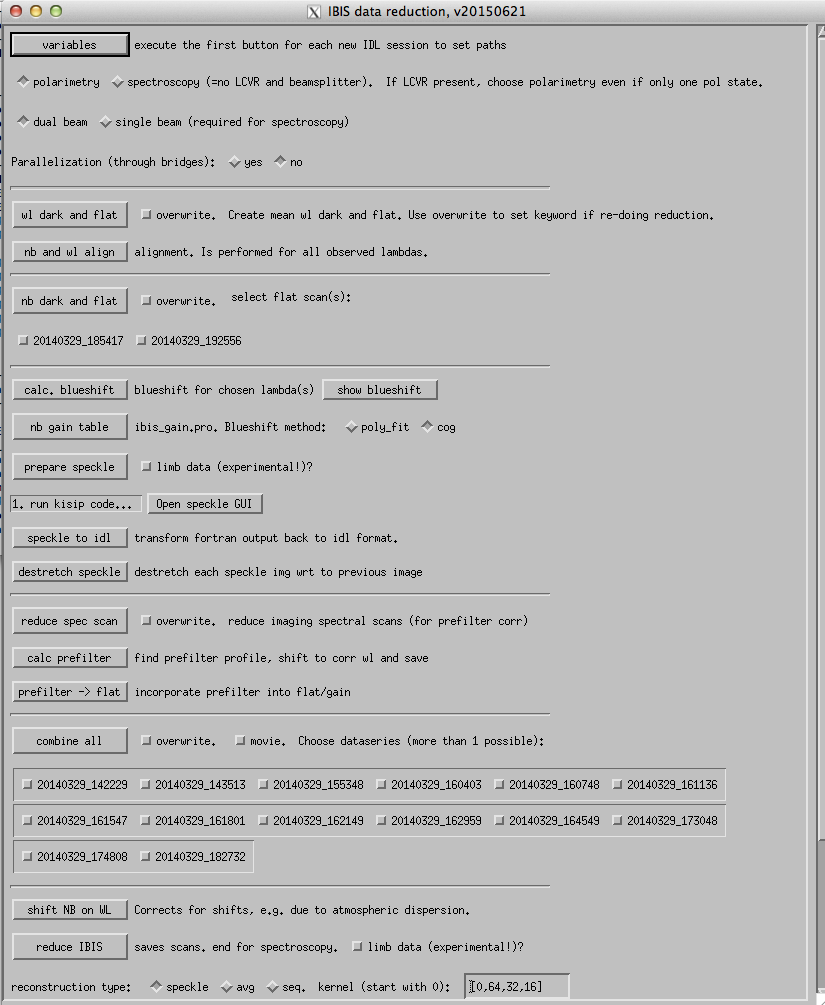
\includegraphics[width=\textwidth]{ibis2.png}
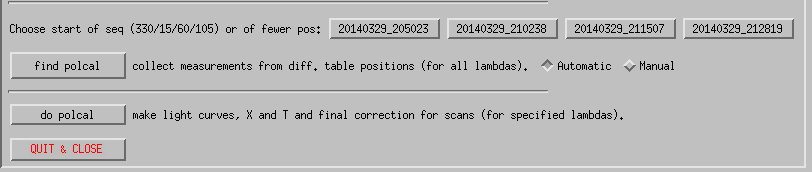
\includegraphics[width=\textwidth]{ibis3.png}
\caption{The IBIS GUI.\label{figgui}}
\end{figure}


\subsection{Variables}

\begin{figure}[htb]
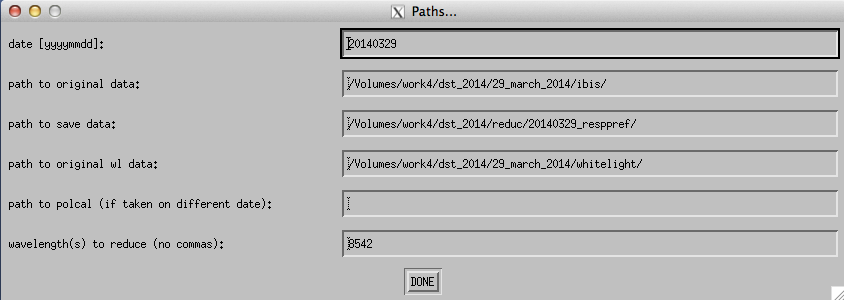
\includegraphics[width=\textwidth]{ibis1.png}
\caption{Variables for the IBIS data reduction.\label{figvar}}
\end{figure}

This is the only input required by the user (see Fig.~\ref{figvar}).\\
\textbf{date}: specify in yyyymmdd format, for example \textit{20110101} \\
\textbf{path to original data}: full path to IBIS data (narrowband) . Subdirectories will be searched.\\
\textbf{path to save data}: full path to save directory (subdirectories created automatically) \\
 The sub-structure that will be created: calibration (for cal files, flats etc.), scans (for combined WL/NB), wl (whitelight and speckle), result\_xxx (final data)\\
\textbf{path to original wl data}: full path to IBIS data (whitelight) . Subdirectories will be searched.\\
\textbf{path to tel.params}: full path to telescope parameters. Pre-2008 the telescope parameters were not in the IBIS headers and a separate camera was run to get them. This line may be left empty for newer data and will not appear in newer GUIs.\\
\textbf{path to linearity corr. curve}: The pre-2010 camera was non-linear and required a linearity correction. May be left empty for newer cameras and will not appear in newer GUIs.\\
\textbf{path to polcal}: If the polcal was taken on a different date, specify its path here in a similar format as 'path to original data'. If this line is left empty, the program assumes that the calibration was taken on the observing data and looks for the subdirectories.\\
\textbf{wavelength(s) to reduce}: for example \textit{6302 8542} or \textit{6302} (no commas)

If you get an error message, try copying ibis\_variables.txt into your current working directory.\\
Calls \textit{textbox\_lk.pro}

This step finds and creates paths and subdirectories. It restarts the GUI afterwards to initialize all measurements found (for example the polcal will go from N/A to actual timestamps).

 Calls \textit{@ibis\_reduce.pro}
  
\subsection{observing mode choices}
\textbf{polarimetry / spectroscopy}: Choose polarimetry if LCVR+PBS were in the beam, even if only Stokes $I$ was measured. Spectroscopy assumes that the FOV is not restricted by the small mask. Several polarimetry programs automatically separate left and right beam. For spectroscopy, stop data reduction after reduce IBIS.

\textbf{dual beam / single beam}: If spectroscopy is chosen, single beam is required. For polarimetry, one may use dual or single beam, although the latter one will be an exception (calibration would be worse and seeing polarization not correctable, but bigger FOV).

\textbf{Parallelization yes / no}: Technically not an observing mode, but mode for data reduction. If yes is chosen, then destretch\_ibis will run in parallel mode. It should be significantly faster, but slightly less stable.

\subsection{wl database -> now obsolete}
Calls \textit{ibis\_wl\_db\_new.pro}

This button will no longer appear in newer version of the GUI.

For the old camera, it constructed a database of sid (seconds into the day) of white-light
images in the directory wl\_dir. This database can then be used
to find the white-light image closest in time to a given narrow-band
image. A structure for the telescope parameters is also created.

pre-2007: telescope parameters from separate camera (kodak headers)
For (early) post-2010 data the database is kept only for compatibility reasons, some variables may be required for speckle. Post-2010 data have the same filename for WL and NB, so the time difference is not used anymore to match the data.

\subsection{wl dark and flat}
Calls \textit{ibis\_wl\_avgdcff.pro}

This program creates a dark and a flatfield image for the whitelight camera. WL data is very simple to reduce and only requires data$_{\rm final}$ = (data$_{\rm orig}$ - dark)/flat, which is performed later.

The program prompts the user for bad scans during darks and flats. Look at the
plot and decide if any datapoints are too low/high. If you do not want
to exclude any scans, simply press enter. Dark image is saved in /calibration/dark\_date.sav.
Flat image saved in /calibration/flat\_date.sav. Examples are shown in Fig.~\ref{figwl}.

\begin{figure}[!htb]
\begin{centering}
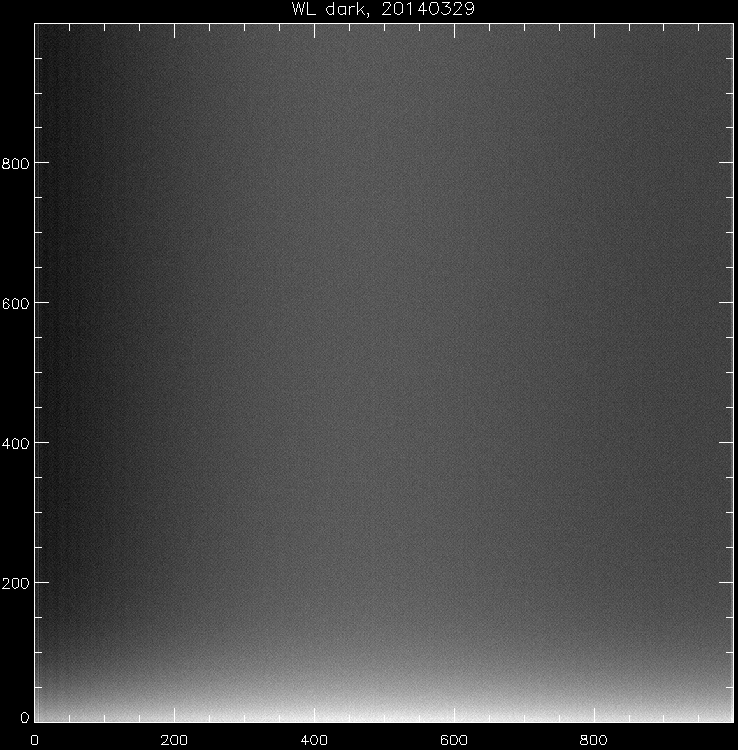
\includegraphics[width=.45\textwidth]{ibiswldark.png}
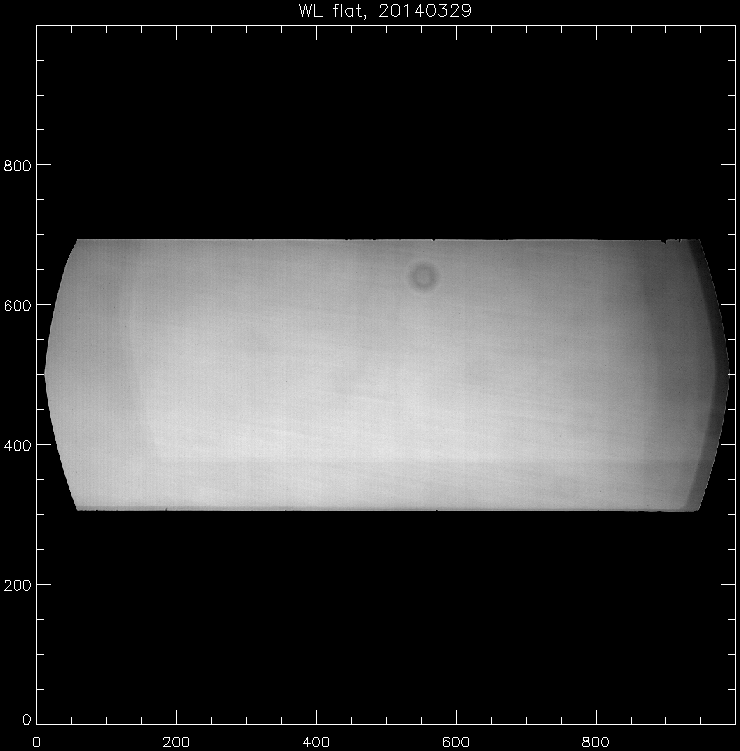
\includegraphics[width=.45\textwidth]{ibiswlflat.png}
\caption{IBIS WL dark and flat.\label{figwl}}
\end{centering}
\end{figure}


\subsection{NB and WL align}
Calls \textit{align\_ibis.pro}.


The two channels, WL and NB, (with different optical paths) need to be aligned exactly so that the destretch can be applied in future steps. This routine is completely different to NSO's version, because it does a crosscorrelation of the whole FOV, not only matching the location of 4 points.

The standard observing sequence includes dot grids and line grids. This program finds all grid files and  does not know by itself if they are dots or lines. Dots seem to work better for the alignment, but lines work too. The USAF target images are not used because they only have characters in the middle of the FOV, which does not lead to a good alignment. Look in your observing log to choose correct series (close in time to observations, because the alignment varies during the day). All observed wavelengths will be aligned, even if not specified in 'variables'.

The program prompts the user to manually rotate/mirror the images (press r) and then save the alignment (press s). This rotation parameter was different for 3 different observing runs and is therefore user-dependent. If you have trouble finding the correct orientation, look for dust on the grid.

Then, user must identify 4-5 corresponding points, first in the left,
then in the right image. This is used as first guess for
auto\_align\_images\_lk.pro. If you cannot select points (clicking has
no effect), it is probably due to a problem with X11 and cursor.pro. This happened on
my Macbook and is described here:\\
http://www.exelisvis.com/Support/HelpArticlesDetail/TabId/219/ArtMID/900/ArticleID/3947/3947.aspx
Enabling "Click-through Inactive Windows" in X11 Preferences solved my issue.

For post-2010 data, the filter and wavelength info is in the header and used to label files correctly. For older data you may need to manually write the corresponding filter and wl into align\_ibis.pro (variables filterindex and filterlist).


requires:\\
 ibis\_mask.pro\\
 avg.pro\\
 diffelement.pro\\
 setpts\_roi.pro (SSW)\\
 setpts\_lk.pro (modified ssw, otherwise contour plots wrong in idl 8.0)\\
 caltrans.pro\\
 auto\_align\_images\_lk.pro (modified SSW for contour plots)\\
 pq2rss.pro (SSW)\\
 anim\_lk.pro (by H. Uitenbroek, modified for modal widgets)


restrictions:\\
The new camera is chosen for observing date 2011 or later. The program
would need to be adapted for observations from aug 2010-dez 2010
 (include month in checks).

Idl 8.0 seems to have a different
contour routine making the plots look strangely compressed. My modified ssw routines
solve this problem.



PS: If one looks at the sequence of grid images during a scan, the grid is moving from image to image. Cannot be due to the AO or the actual glass plate. Possibly temperature variations? Therefore, the program uses the same extension in WL and NB for the crosscorrelation and only one image (no averaging, which would smear the dot pattern).

New in 2014: now all NB data will be aligned with respect to the broadband data. This has the advantage that final NB data should not require any cross-alignment (though a shift may be introduced by the destretch).

Updated in 2017 for single/dual beam. The offset of L/R beam is set to 0 in the single-beam case. The first guess looks bad for single beam (again issue with contour routine?), but the alignment seems to work.

\subsection{nb dark and flat}
Calls \textit{ibis\_dark\_avg\_nb.pro} (new cam). One dark array per filter is created.

Calls \textit{ibis\_flat\_avg\_nb.pro} (new cam).

This routine creates the dark and flatfield images for the narrowband data. The dark is one image per wavelength (even though it probably does not depend on wavelength). 

The flat scans need to be selected from the suggested timestamps in the GUI. Use at least 30 scans. For the old cam, one needs to specify nmax if the scans were aborted. Otherwise the program crashes reading a shorter-than-expected logfile. This option is not shown and unnecessary for the new cam because files are searched with file\_search() and aborted series do not matter. The output is a flat array where equal wavelengths and stokes states are averaged into one image.

\subsection{calc.~blueshift}
Calls \textit{ibis\_blueshift.pro}.

This routine calculates the blueshift of the instrumental profile (redshift of the spectral lines) induced by the collimated mount of the Fabry Perot. It uses flatfield data.

Procedure: load nb flat and dark, order flat by ascending wavelength, average all images of same wavelength and polarization state. Updated flat is saved, old flat is now called .backup. The user manually selects a wavelength range to use for blueshift calculation (once per prefilter) to avoid double lines as in 6301/6302. Calls \textit{ibis\_blueshift\_map.pro} to get the actual blueshift.

Blueshift calculation:\\
- Wavelength scale is interpolated to 10 m\AA\ grid. Data are interpolated (quadratic) on this scale. Left and right beam are treated separately.\\
 - Find line center for each pixel (COG, poly\_fit)\\
-  surface fit for this map, (average all fits for each pol. state -> one map per filter)\\

\begin{figure}[!htb]
\begin{centering}
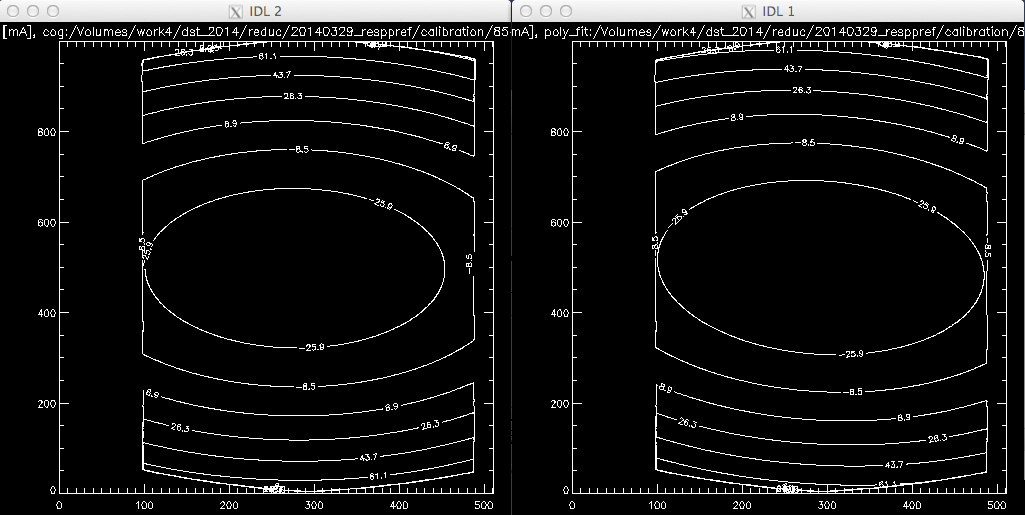
\includegraphics[width=.9\textwidth]{ibisblueshift.png}
\caption{IBIS blueshift example for 8542 \AA. Left: COG calculation, right: poly\_fit. \label{figbs}}
\end{centering}
\end{figure}

 
Loops through wavelengths chosen in 'variables'. If a blueshift for a certain wavelength already exists, the program asks if it should be overwritten.

The maps can be viewed with the button on the right that calls \textit{view\_blueshift.pro} and an example is shown in Fig.~\ref{figbs}. 

\subsection{nb gain table}
This routine calculates the gain table of the narrowband data. The nb gain needs to be constructed without influence from the blueshift, which is why the blueshift needs to be calculated earlier and removed in this routine. Otherwise the gain would show concentric rings in the FOV.

Choose which blueshift file should be used: poly\_fit (=polynomial fit) or COG (center-of-gravity). COG seems to be more stable if the camera has fringes or if the line is as broad as 6563.

Calls \textit{ibis\_gain.pro}

Procedure:\\
 - interpolate wl of each pixel in flat to common 10 m\AA\ scale -> average FOV -> get one flat profile\\
 - make shifted map of this average profile\\
-  difference between left and right beam (cfactor)\\
-  flat without spectral lines: measured flats / (shifted avg profile map)


Update June 2015: The ``bad'' profile is now constructed from a 100x100 px box centered in the mask (with no error catching if this box ends up where it shouldn't, since I want the program to crash then to find the error). This ensures that variations due to the blueshift of the prefilter transmission profile are taken care of automatically.

\subsection{prepare speckle}
\label{prepspeckle}
Calls \textit{ibis\_reduce\_speckle.pro} or \textit{ibis\_reduce\_speckle\_ncam.pro} 

For the post 2010 camera, there currently is one speckle file per ibis file. The burst size is given by the number of extensions with same filter. I.e.~ if one observes 20 wavelengths of 6302 (polarimetry) and 15 wavelength of 6563 (Stokes $I$ only), then the burst size for 6302 will be 20*6 and for 6563 only 15, which is too low for a good speckle. The ideal size is around 70 files / burst.

So far, there is no way to save multiple files of same timestamp or to combine different files for a larger burst size. Also the program will probably crash if anybody used the repeat option (R>1) while observing. This would be a major change, because it makes finding the correct reconstruction for an observation much harder.

The program creates all ibis\_wl\_* files, which are in binary little-endian format. They only contain the actual image, whose size will be smaller than the 1000x1000 chip size.

Creates speckle\_dims.txt and speckle\_sid.sav which contains speckle\_db.

The parameters for speckle are saved in speckle\_dims.txt. Look for the pixel size of the image, and the images per burst for each wavelength in the lower part of that file. speckle\_db is necessary for destretch speckle.

todo: create input files for speckle automatically.

Speckle needs to be run manually! If you do not do speckle, you can omit sections \ref{prepspeckle} - \ref{destrsp} and continue with combine and choose 'avg' or 'seq' for alignment later.

\subsection{Open speckle GUI}
\label{sgui}

There is a speckle GUI written by Fred, which uses GraphApp commands. I could not get it to compile on Mac OSX.
This GUI does exactly the same (creating the 3 files init\_file.dat,
init\_method.dat and init\_props.dat), but has additional options to
display the reconstructed data. 

One may also launch the speckle reconstruction from the last tab in
the program. Be sure to set the image size, the number of images (from
speckle\_dims.txt) and
the number of speckle files in the appropriate fields.

To do: read speckle\_dims.txt and make speckle automatic


\subsection{speckle to idl}
\label{stoi}
Calls \textit{ibis\_prepare\_speckle.pro}.

Converts speckle binary files (*.final) to IDL save files (*.sav). Their original size (usually 1000x1000) is restored.

\subsection{destretch speckle}
\label{destrsp}

Calls \textit{ibis\_detr\_speckle.pro} (own program).

This program destretches all speckle images. First, it finds all *.sav images, then it orders them by time using info from speckle\_db. When the timestamp changes, the program checks by cross-correlation if the same target was still observed and if yes, the destretch continues. Otherwise it starts a new destretch round with the first image of the series being the reference. The reference image keeps changing throughout the series to take solar evolution into account. The program overwrites all *.sav files to save space. The original *.sav files can be recreated fast with `speckle to idl'.

The program only works with post-2010 cam data. The older data that I have already looked good without it.

A hard-wired kernel of  ds\_kernel = [0,64,32] is used. It is probably not perfect, especially for data with bad seeing, but adding another level would be much slower.


\subsection{reduce spec scan}
Calls \textit{read\_imagingspecscan.pro}

Finds all imaging spectral scans, asks which one to use if multiple are found. Dark-corrects (watch the exposure times!) and blueshifts the spectral scan data to be able to get a single average profile of the spectrum convolved with the prefilter transmission.

The average profile and a relative wavelength scale are saved in calibration/ imgspecscan\{wl\}.sav

Warning: The program will crash if the images are not 1000x1000 or larger. One needs to change xl, xr, y1 and y2 in the routine to redefine the area to be averaged for other image sizes.

\subsection{calc prefilter}
Calls \textit{ibis\_corr\_prefilter.pro}

The goal is to find the shift of the prefilter profile, which was measured by the PMT and thus has a different optical path and a relative wavelength offset to other data. The steps are:\\
1) broaden atlas by IBIS FWHM and shift atlas to correct minimum (strangely, my copy of the FTS atlas has a 40 m\AA\ shift of the 8542.1 line for example)\\
2) Cross-correlate flat to atlas for wavelength-offset of the data\\
3) compare info\_flat\_short.grid and info\_flat\_short.wave (relative/absolute wl) to find offset to absolute wl (wscale)\\
4) shift prefilter relative to spectral scan for best match (crosscorrelation) with atlas\\
5) save prefilter wl scale (new) and prefilter transmission

Warning: So far, this routine is only useful for 6302, 6563, 8542, 6173, 5434. For other lines, the program would require a prefilter file (done by Kevin and available in directory, but not ready to use) and some modifications (hardwired) such as the wavelength of the theoretical line center in air, an optional wavelength shift of the FTS atlas, and setting the region for cross-correlation manually (to exclude telluric lines for example).

Note that the fringes of the prefilter are not taken into account currently. It is therefore normal to see a sinusoidal continuum with an amplitude variation of ~2\% in the final data. This would require implementing a crosscorrelation with the fringe pattern derived by Kevin.

\subsection{prefilter -> flat}
Calls \textit{flat\_prefilter.pro}

For each lambda, this program finds the gain file, the prefilter file and overwrites (!) the previous gain by
$$gain = gain / ip\_pref $$ where ip\_pref is the prefilter profile interpolated at the observed wavelengths.
This process ensures that the prefilter correction is applied to the data automatically when the gain table is applied. It has no influence on X-matrices or response matrices, because they are normalized to their first element, meaning that the intensity stays constant.

An info variable is added to the corrected gain files to avoid future prefilter corrections.



\subsection{combine all}
Calls \textit{ibis\_combine\_ncam.pro} 
Calls \textit{assign\_speckle2nb\_ncam.pro}.

For the selected timestamps, this creates idl save files of the scans
in the \textit{temporary} directory. Darks and flatfields are also
applied. This is done for ALL observed wavelengths, independent of your selection of variables. In case this step crashes in the middle, you will need to set 'overwrite' to redo it.

A speckle database is created so that reduce IBIS can figure out which
speckle file (those only have numbers 000, 001, 002, ... instead of
actual timestamps) corresponds to the current data.

Note that if the gain was not corrected for the prefilter, this step will still work. But it is best to create gain files and prefilter profiles for all observed wavelengths (to be set in variables), before doing this step.


\subsection{shift NB on WL}
Calls \textit{ibis\_shiftatmosdisp.pro} 

Discovered on 20140306 that the alignment of the target images only is good for rotation and scaling. In the science data, there is an extra shift between NB and WL data, probably due to atmospheric dispersion. It can reach up to 15 pixels in the mornings and evenings according to a calculation by Kevin. Shifts of 11 px were easily found. Therefore, one needs to crosscorrelate the NB data directly to the BB data, which needs to be done in the photospheric line wing to have similar features. 

This routine will restore the sav files created by 'combine' and check if the variable atmshift already exists in the file. If yes, then the correction was already done, but otherwise the user will have to interactively determine if the crosscorrelation is sufficiently good. So far, this is done for every single file manually, because we are not sure yet how much of a drift to expect with time.

Note: There are two different opinions whether this step is needed. If the turbulence occurs close to the telescope, then this step may need to be omitted because the turbulence should depend on the pixel location on the camera and not the solar region. In this case, one should do the destretch applying the same vectors to the same pixels in 8542/6302 (independent of the solar features there) and find the shift due to dispersion between the wavelengths after the destretch. However, because the seeing depends on wavelength anyway, both options may not be great and the shifts may need to be scaled down for longer wavelengths. I have never compared any of these options.


\subsection{reduce IBIS}
Calls \textit{ibis\_calibrate.pro}

This program does the actual destretch, blueshift correction, and
alignment of the files in the chosen directories. The results are
saved in the timestamp-subdirectories from where the reduction is performed.

This part uses the timestamps that are checked above in the GUI and the 'cog' or 'poly' method for the blueshift. 'cog' works better for 8542 and 6563, 'poly' works better for 6302. Therefore, it is recommended to run this step twice with different entries in 'variables' and selecting the appropriate blueshift method for the selected wavelength.

April 2017: Dual beam polarimetry and single beam spectroscopy are tested and should work. Single beam polarimetry does not work (not tested, not adapted) and currently has 'stops' in my places. Single beam spectroscopy is not parallelized (bridges and no\_bridges routines are identical).

\subsection{find polcal}
Calls \textit{collect\_ibis\_polcal.pro}

Creates subdirectories polcal\_xx that contain one file per wavelength per calibration sequence (000-027). These files contain nb\_data = [x,y,stokes*wavelengths]. The number of wavelengths here is low (5-6) since the polcal is assumed to be constant over the spectral line and it can be run much faster without too many wavelength points.

Make sure that you check the observer's log to see if any polcal was
aborted. In this case, select the correct timestamps
before you press 'find polcal'.

\subsection{do polcal}

User first needs to select which directories to calibrate. Program then displays red boxes denoting the FOV of the left and the right beam. If those looks ok (should be most of the time), press (a), otherwise press (c) and click on lower left then upper right of L beam, then lower left or R beam.

The proper T-matrix (telescope calibration) is chosen automatically by date of observation.  The newest one is from May 2010 and the mirrors most likely have been recoated since, but no newer file is available [in July 2016].

 Calls \texttt{ibis\_get\_polcalcurvec}. This program first finds all sav files in the polcal subdirectories. Not all 4 table positions are required, even with 2 positions, the calibration is the same. First, the darks are subtracted from the polcal. Then, the data are put into the state [1. , state2/state1, state3/state1, state4/state1, state5/state1, state6/state1]. This means that 6 modulation states are hardcoded and that only the normalized Muller matrix of the instrument is determined. One assumption for the cal is that the lightlevel remains constant during the measurement of the six modulation states. Intensities at each y-pixel are kept, while one averages over x-pixels, i.e. the response matrix will be determined for each pixel along the long axis of the IBIS FOV. The telescope info and the polcal intensities are saved in  e.g. calibration/20140329\_polcal\_8542.sav.
 
Note November 2014: X is calculated for y-pixel and wavelength now, but the average of the FOV is still being used for the polcal (found no real improvement by using y-dependent X matrix).

The next routine called is  \texttt{ibis\_polcal\_xcalc\_v4}. Its goal is to derive the response matrix, i.e. the 4 $\times$ 6 matrix $X$, which transforms the observed modulated intensities $S'$ (I+Q, I-Q, I+V, I-V, I+U, I-U, however the names of the states have nothing to do with the actual polarization state) into the solar S (I, Q, U, V). 
\begin{equation}
S' = X T S
\end{equation}
 The telescope matrix $T$ is used during the fitting. The actual fitting is done with mpfitfun, which is run in parallelized mode for each wavelength point (by calling \texttt{aux\_xcalc\_v4}), otherwise it would take $>$1h for the usually 6-7 wavelength points. There are 28 free parameters: 24 matrix entries, the waveplate offset, the waveplate retardance, the waveplate dichroism and the linear polarizer extinction. One may have to install for\_split.pro to make the parallelization work. The output is saved as e.g. 01.ta.20140329.8542.X.idl for the left beam and 01.tb.20140329.6302.X.idl for the right beam. The dimensions of xmat are Array[4, 6, 903, 8], meaning 4x6 matrix for 903 y-pixels and 8 wavelength points.

The main program (IBIS GUI) then queries the user for a region of quiet Sun, later to be used for crosstalk calibration. Savefile: \texttt{qsreg.txt}. If the file already exists, the QS region is not displayed anymore.

The IBIS GUI then queries for the choice of continuum (choose left edge and right edge, ideally 2 wavelength points) and saves it in cont\_8542\_sav.

For the actual calibration of the data, \texttt{main\_ibis\_calibrate\_v2} is called. It restores the response matrices for both beams and the T-matrix and calls several subprograms: 


\begin{minipage}{0.05\textwidth}\hfill
\end{minipage}
\begin{minipage}{0.95\textwidth}
It calls \texttt{ibis\_scan\_calibrate\_xt\_v2}, which by default averages the X-matrices over y-pixels (other options include smoothing and linear fitting should be implemented) and wavelength. It then inverts the 4x6 matrix via SVD and interpolates it for each observed wavelength step (which has no effect, since the wavelengths were averaged, but this could be used for wavelength-dependent X-matrix calibrations). The telescope matrix is 4x4 and is inverted with INVERT().
The program then loops over all pixels and calculates $T^{-1} \#\# X^{-1} \#\#$ pixel, giving the normalized observed Stokes vector (I, Q, U, V). Left and right beams are then combined as
\begin{eqnarray*}
I = 0.5 * (I_L + I_R) \\
Q = 0.5 * ((Q_L / I_L) + (Q_R/I_R)) * I \\
\cdots
\end{eqnarray*}
to account for different beam intensities (beam balancing).

If the keyword region is set (by default it is), then the quiet Sun is used to correct for I$\rightarrow$Q,U,V crosstalk via \texttt{ibis\_scan\_xtalk\_i2quv}. The continuum points that the user chose are used to average to a continuum value of I,Q,U,V. For the QS region that the user selected, the fractional polarizations Q/I, U/I and V/I are calculated (in the continuum). Those are the values polfac = [polfacv, polfacq, polfacu] that are also saved later. The corrections for the crosstalk calculates e.g. V$_{new}$ = V - polfacv $\cdot$ I. Note: the residual crosstalk (V$\rightarrow$Q,U and Q,U$\rightarrow$V) is not corrected, because it led to strange results and shall be done manually if necessary.

Q and U are then rotated into the correct solar reference frame, which depends on the solar P angle and uses a calculations that I have no clue of what it does.

The calibrated data are saved as e.g. 6302\_nb027.pc.tatb.sav, pc standing for polcal and tatb for both beams. This is the final step of the pipeline.

\end{minipage}








%\subsection{do prefilter corr}
%Calls \textit{apply\_prefilter.pro}
%
%Overwrites (!) all reduced data with a new, corrected stokesout. Basically, stokesout$_{\rm new}$ = stokesout$_{\rm old}$ / (prefilter, interpolated at correct wavelengths). This is done for all polarization states. An info variable is added to the corrected files to avoid future prefilter corrections.

%This part uses the timestamps are are checked above in the GUI.



\section{Versions and changes}

v170413
\begin{itemize}
\item Adapted and tested pipeline for single-beam. Many functions were adapted. No changes to dual-beam methods, apart from finding bug in atmospheric dispersion routine (atmosdisp), which only applied shifts to L beam in the past and not R beam.
\end{itemize}


v150621: June 2015
\begin{itemize}
\item Until now, the prefilter correction was applied as a last step. This is incorrect, because it should be applied before the demodulation. Also, the spatially varying (blueshifted) prefilter transmission profile needs to be taken into account. Therefore, construct the ``flat'' profile only from a small box (100 x 100 pixels around the center of the mask), otherwise the prefilter transmission changes would be divided out. The prefilter correction is now applied to the gain, which will automatically correct the data. Note that differences to data with the old prefilter correction are minimal, especially near the center of the prefilter (where the spectral line usually is).
\item Fixed possible crash if user selected wrong corner for rigid alignment feature
\item All prefilter files are now available, but not implemented (requires changing variable names and some hard-wired parameters, such as locations of telluric lines). Currently, the prefilter correction works for 8542, 6302, 6173, 6563, 5434. Let me know if you need another filter.
\item Updated manual in March 2016 to contain some figures and examples.
\item Updated manual in July 2016 to explain polcal in detail.
\end{itemize}


v141114: November 2014
\begin{itemize}
\item Polcal was found to depend on spatial y (long axis of IBIS mask) and wavelength, especially far from line center. Now X-matrices are computed with more dimensions and less averaging. Implemented parallelization of X-computation. The spatially dependent X-matrix however did not solve the calibration issues for 6302 on 20140329. For 8542, a constant matrix has always worked. Therefore, the default is currently to still calculate and save the spatially dependent X, but then average over the FOV and only apply one X-matrix per beam (can be modified in main\_ibis\_calibrate\_v2.pro:84 by removing the /avg keyword).
\end{itemize}


v140221: January/Feb 2014
\begin{itemize}
\item Support for old camera dropped (use v5 for that).
\item Alignment done with respect to whitelight images. All wavelengths should thus be aligned.
\item speckle\_gui implemented that can run the speckle code and display reconstructed images
\item GUI is now based on pointers instead of common variables.
\item Polcal should work with fewer than 4 table positions. 2 are
  recommended, 1 is required.
\item Atmospheric refraction was discovered to be significant. Now NB data can be correlated to WL data for each scan.
\end{itemize}



v5: 2013
\begin{itemize}
\item More or less stable reduction.
\end{itemize}



v4: May 4, 2012:
\begin{itemize}
\item completely cleaned up the ibis\_v4\_lucia directory. Now it should contain all necessary routines to run the reduction.
\item substituted the old ASP cal with a new polcal written by T. Schad. The old cal required many more routines, was a lot less understandable and the resulting X matrices are the same in both versions.
\item Enabled logging. A .tex log containing  each performed step is saved in the \textit{log} subdirectory.
\item Many bug fixes, especially for the old camera, but also for the alignment procedure and the beam combination (beam balancing by T. Schad). The region for the polcal is now guessed by the program. The region for rigid alignment is now saved for each timestamp, not globally.
\item T. Schad implemented a parallelization of the destretch using IDL bridges. The default setting is off in the GUI because it might be a little unstable, but it can be enabled by checking the box.
\end{itemize}

v3: 2012:
\begin{itemize}
\item implemented prefilter correction
\end{itemize}

\section{Bibliography}


\end{document}
